\chapter{検出手法の設計と実装}
\section{研究背景}
\subsection{開発の経緯}
RNA editingとは、転写物へ位置特異的に一塩基置換を引き起こす転写後修飾の一種として知られ、アデニン (A)からイノシン (I)へのA-to-I editingがヒトやマウス、ショウジョウバエから多数報告されている。このA-to-I editingはADARと呼ばれる二本鎖RNA結合タンパク質によって触媒されることが知られており、翻訳の段階で置換されたイノシンはグアノシンとして認識されるため、editingを受けた転写物は翻訳の過程において、非同義置換によるスプライシングサイトの変化やタンパク質の高次構造の変化、microRNAへのeditingを介した遺伝子発現の抑制など転写調節に幅広く関与していることが報告されている。近年、RNA-seqデータを用いたゲノムワイドなeditingサイトの同定が多数の組織およびセルラインを用いて行われ、ヒトでは数万箇所のeditingサイトが報告されている。RNA editingサイトはゲノムと転写物の一塩基のミスマッチとして検出可能だが、シーケンシングやマッピングに起因した擬陽性を多く含むため、真のeditingサイトと擬陽性を高精度に分離する検出手法がこれまで多く提案されている。しかしながら、解析に使用された手法の多くはソフトウェアとして公開されておらず、RNA-seqデータを対象としたeditingサイトの検出ソフトウェアは現時点で一つ存在するのみである。そこで本研究では、既存のソフトウェアよりも高速かつ低メモリで動作し、アラインメントデータへの統計的なフィルタリング手法、実験デザインを考慮した解析を可能にするRNA editingサイトの検出パッケージの開発を行った。本パッケージは、既存のソフトウェアと比較して高速か低メモリで動作し、付属するベンチマーキングツールによって、検出したeditingサイトの検出精度を定量的に評価することを可能にした。尚、本パッケージは、GPLの元、オープンソースのフリーウェアとして公開することを予定している。

\subsection{要求分析}
現在、RNA-seqデータからRNA editingサイトを新規に検出する手法は、REDIToolsの一つの実装に限られている。
\par
こういった背景から本研究では、以下の内容を含んだソフトウェア・パッケージ、Ivyの設計と実装を行った。
\begin{enumerate}
	\renewcommand{\labelenumi}{(\roman{enumi})}
	\item RNA-seqデータから高速かつ高精度にRNA editingサイトを検出するソフトウェア
	\item 本ソフトウェアにより検出された新規RNA editingサイトの検出精度を評価するベンチマークツール
\end{enumerate}

\section{設計と実装}
\subsection{システムの設計}
IvyはUnix環境で動作するコマンドラインツールとして開発され、Pythonによって実装されている。入力で与えられたSAM/BAMファイルは、Pysam (Python interface for the SAM/BAM sequence alignment and mapping format)ライブラリを使用して参照ゲノムへのアラインメント結果を取得している。Pysamは、Cで書かれたSAM/BAMのパーサー (Samtools C API)とのバインディングであり、Pythonのインターフェースから高速にアラインメント情報を取得可能であることから採用した。
Ivyは、ソースコードに同梱されているインストールスクリプトが必要なライブラリを自動的にコンパイル、インストールするため、コマンド一つで容易にインストールすることが可能となっている。またIvyはPyPi (Python package index)への登録を予定しており、将来的にはソースコードのダウンロードも不要となり、コマンド一行のみで使用可能になる予定である。
\par
以下に、本研究によって開発されたシステムの設計を示した。
\begin{figure}[htbp]
	\begin{center}
		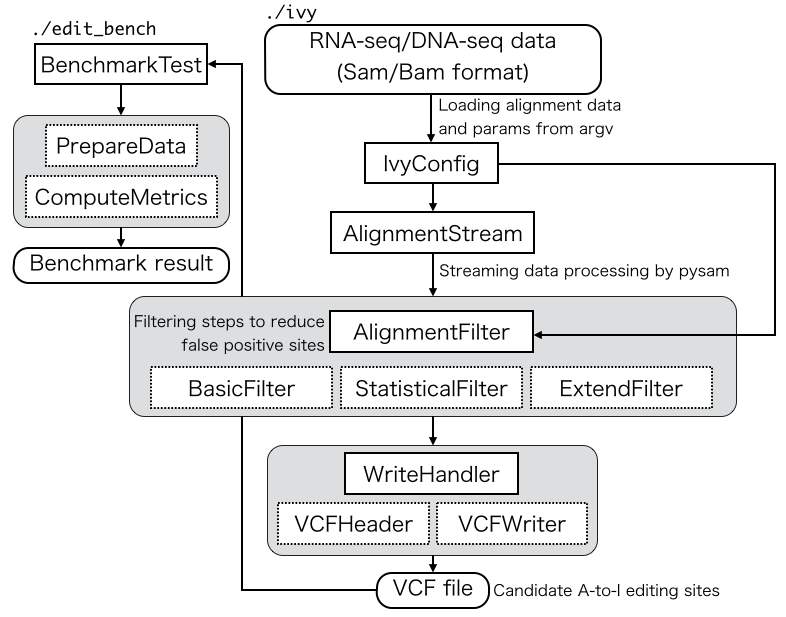
\includegraphics[width=0.7 \hsize]{Ivy_arch.png}
	\end{center}
	\vspace*{-1cm}
	\caption{Ivyのシステム}
\end{figure}

\subsection{データの入出力}
\subsubsection{SAM/BAM形式による入力}
超並列シーケンサーを用いた解析において、塩基配列データはFastqフォーマットが標準的な形式となっており、fastqデータを参照ゲノム配列にマッピングすることによって、SNPの検出や遺伝子発現量の定量、ゲノムのアセンブリなどが行われ、RNA editingサイトの検出も参照ゲノムへのマッピングが検出には必須である。このマッピングしたアラインメント結果を保持するデータ形式は、SAM/BAM形式が事実上の標準フォーマットとして広く用いられている。SAMは参照ゲノムへマッピングされたショートリードの座標情報やクオリティ情報などを保持しており、座標にインデックスを貼りgzipで圧縮したバイナリ形式をBAMと呼ぶ。SAMとBAMは相互に変換が可能である。Ivyは、入力には参照ゲノムにマッピングしたSAMもしくはBAMを入力フォーマットとした。

\subsubsection{VCF形式による出力}
Ivyによって検出されたA-to-I editingサイトは、VCF (variant call format)によって出力される。このVCFフォーマットは、SNPやSNVの検出といった変異解析に標準的に用いられているフォーマットを指し、1000 genomes projectなど国際プロジェクトでも採用されているデータ形式である。RNA editingサイトもSNPも本質的にはゲノムのある座標における一塩基置換として表現可能であるから、検出したRNA editingサイトもVCF形式で出力することが望ましいと考えた。VCFを出力フォーマットとする利点として、変異解析のために開発された他のミドルウェアを組み合わせた更なる解析が可能となる点である。SNP解析では検出したSNPそれぞれの遺伝子名やアミノ酸置換の有無などをAnnovarとったソフトウェアを用いてアノテーションする場合が多い。Ivyで出力された結果もまたVCFであるから、Annovarなど他のツールと連携させた下流解析を容易に行うことができるという利点を持つ。
\par
以下に、VCFフォーマットによる結果の出力例を示す。

\scriptsize
\begin{verbatim}
##fileformat=VCFv4.2
##INFO=<ID=NS,Number=1,Type=Integer,Description="Number of Samples With Data">
##FILTER=<ID=s50,Description="Less than 50% of samples have data">
##FORMAT=<ID=GT,Number=1,Type=String,Description="Genotype">
#CHROM POS   ID        REF ALT QUAL FILTER INFO                    FORMAT      NA00001        
20     14370 rs6054257 G   A   29   PASS   NS=3;DP=14;AF=0.5;DB;H2 GT:GQ:DP:HQ 0|0:48:1:51,51 
20     17330 .         T   A   3    q10    NS=3;DP=11;AF=0.017     GT:GQ:DP:HQ 0|0:49:3:58,50 
\end{verbatim}
\normalsize

\subsection{並列化への対応}
Ivyは、ヒト、マウス、ショウジョウバエといった高等真核生物をターゲットとしている。Ivyはゲノム全体についてeditingサイトの検出を実行するため、ゲノムサイズが大きな生物に対しては計算時間が増大することが想定され、複数のスレッド (CPU)を使用した並列化が高速な解析には必要となる。Ivyでは、検出の高速化のために使用可能なスレッド数に応じ、自動的に染色体数を均等に分割し、並列的にeditingサイトを検出する並列処理をサポートしている。RNA editingサイトは、染色体をまたいで起こる現象ではないため、染色体を分割することによるアラインメントデータの損失などの問題は起こらないと考えられた。

\subsection{ユーザーインターフェース}
Ivyパッケージに同梱されるivyコマンドはRNA editingサイトの検出ソフトウェアであり、edit\_benchは検出したeditingサイトの精度検証を行うことのできるベンチマークツールである。
ivyのインターフェースは以下のようになっており、同梱されているサンプルデータを用いて解析を簡易的に試すことができるようになっている。
\par
Ivyパッケージは、以下のコマンドで容易にインストールすることが可能となっている。
\begin{itembox}[l]{Ivyのインストール}
	\begin{verbatim}
		#最新版のソースコードの取得
		$ git clone git@github.com:soh-i/Ivy.git 
		#パッケージのインストール
		$ python setup.py install
	\end{verbatim}
\end{itembox}

edit\_benchは、以下のように使うことが出来る。
\begin{itembox}[l]{ivyのインターフェース}
	\begin{verbatim}
		$ ivy -f reference.fa -r dna.bam --rm-duplicated-read --insertion-read
	\end{verbatim}
\end{itembox}

\par

edit\_benchは、以下のように使うことが出来る。

\begin{itembox}[l]{edit\_benchのインターフェース}
	\begin{verbatim}
		#基本的な使い方
		$ edit_bench --vcf test.vcf --sp human_hg19 --plot --log bench.log

		#正解セットのカスタマイズ
		$ edit_bench --vcf test.vcf --sp human_hg19 --source brain \\ 
		  --log bench.log
	\end{verbatim}
\end{itembox}

\section{本手法の性能評価}
\subsection{性能評価に用いたRNA-seqデータ}
\subsection{使用したパラメータ}
\subsection{性能評価の結果}
\subsection{実データを用いたRNA editingサイトの解析}

\section{議論}
\subsection{本手法により同定されたeditingサイト}
\subsection{本手法の有用性}
